\documentclass[preprint,12pt]{elsarticle}

%% Packages
\usepackage{amsthm,amsmath,amsfonts,amssymb}
\usepackage{mathtools}
\usepackage{graphicx}
\usepackage{booktabs}
\usepackage{array}
\usepackage{flafter}
\usepackage{placeins}
\usepackage{microtype}
\usepackage{etoolbox}
\usepackage{needspace}
\usepackage[colorlinks=true,linkcolor=blue,citecolor=blue,urlcolor=blue]{hyperref}

\makeatletter
% Expandable table input keeps alignment rules valid after generated rows.
\let\inputresultrows\@@input
\setlength{\@fptop}{0pt}
\setlength{\@fpsep}{12pt plus 2pt minus 2pt}
\let\ps@pprintTitle\ps@plain
\makeatother
\pretocmd{\section}{\Needspace{6\baselineskip}}{}{%
  \PackageError{revision-layout}{Section spacing patch failed}{Check the document class.}}
\patchcmd{\pprintMaketitle}{\vskip36pt}{\vskip12pt}{}{%
  \PackageError{revision-layout}{Title spacing patch failed}{Check the document class.}}
\patchcmd{\pprintMaketitle}{\vskip18pt}{\vskip12pt}{}{%
  \PackageError{revision-layout}{Title-author spacing patch failed}{Check the document class.}}
\patchcmd{\pprintMaketitle}{\unvbox\absbox\par\vskip10pt}{\unvbox\absbox\par\vskip4pt}{}{%
  \PackageError{revision-layout}{Abstract spacing patch failed}{Check the document class.}}
\renewcommand{\topfraction}{0.9}
\renewcommand{\bottomfraction}{0.8}
\renewcommand{\textfraction}{0.07}
\renewcommand{\floatpagefraction}{0.85}
\setcounter{topnumber}{3}
\setcounter{totalnumber}{4}
\setlength{\textfloatsep}{10pt plus 2pt minus 2pt}
\setlength{\floatsep}{8pt plus 2pt minus 2pt}
\setlength{\intextsep}{10pt plus 2pt minus 2pt}
\setlength{\abovecaptionskip}{4pt}
\setlength{\belowcaptionskip}{2pt}
\setlength{\bibsep}{0pt plus 0.3ex}

\journal{Statistics in Biosciences}
\biboptions{authoryear,round}
\hypersetup{
  pdftitle={Randomized Kolmogorov-Smirnov Calibration for Fitted Discrete Single-Cell Residual Diagnostics},
  pdfauthor={Elvis Han Cui, Yihao Li, Zhuang Liu}
}

\newcommand\E{\mathbb{E}}
\newcommand{\Prob}{\mathbb{P}}
\newcommand{\Cov}{\operatorname{Cov}}

%\numberwithin{equation}{section}

\theoremstyle{plain}
\newtheorem{axiom}{Axiom}
\newtheorem{claim}[axiom]{Claim}
\newtheorem{theorem}{Theorem}[section]
\newtheorem{lemma}[theorem]{Lemma}
\newtheorem{corollary}[theorem]{Corollary}
\newtheorem{proposition}[theorem]{Proposition}

\theoremstyle{remark}
\newtheorem{definition}[theorem]{Definition}
\newtheorem{remark}[theorem]{Remark}
\newtheorem{algorithm}{Algorithm}
\newtheorem*{example}{Example}
\newtheorem*{fact}{Fact}

\begin{document}

\begin{frontmatter}
\title{Randomized Kolmogorov--Smirnov Calibration for Fitted Discrete Single-Cell Residual Diagnostics}

\author[zju,ucla]{Elvis Han Cui\corref{cor1}}
\ead{elviscuihan@g.ucla.edu}
\cortext[cor1]{Corresponding author.}

\author[zju,genentech]{Yihao Li}
\ead{li.yihao@gene.com}

\author[zju,google]{Zhuang Liu}
\ead{zhuangl@google.com}

\affiliation[zju]{organization={College of Environmental and Resource Sciences, Zhejiang University},
            city={Hangzhou},
            country={China}}

\affiliation[ucla]{organization={Department of Biostatistics, University of California, Los Angeles},
            state={CA},
            country={USA}}

\affiliation[genentech]{organization={Genentech},
            city={South San Francisco},
            state={CA},
            country={USA}}

\affiliation[google]{organization={Google},
            city={Mountain View},
            state={CA},
            country={USA}}

\begin{abstract}
Residual diagnostics for discrete single-cell models often reuse the data used
to fit a count margin, trend, or simulator. \emph{Calibration} means choosing
a reference law that preserves the nominal false-positive rate for this fitted
procedure. The ordinary Kolmogorov--Smirnov (KS) reference generally fails
because it treats the null distribution as fixed. We specify a randomized
residual workflow that separates marginal, covariate-indexed, and dependence
diagnostics and repeats simulation, fitting, and residual construction in the
bootstrap. Classical composite-null empirical-process theory supplies the
justification. Known discrete margins yield independent uniform residuals for
independent observations; regular fitted margins yield a plug-in Gaussian
limit, targeted by the bootstrap under corresponding consistency conditions.
Separate gene-wise marginal KS tests cannot detect copula-only errors.
Simulations through 10,000 observations show persistent miscalibration of naive
references and near-nominal rejection after refitting. scGTM and scDesign3
examples illustrate distinct residual targets, while public IMvigor210 PBMC
data expose discrepancies from a patient-and-depth conditional working model.
The contribution is a discrete-residual specialization of established theory
with explicit limits for complex fitted models.
\end{abstract}

\begin{keyword}
Kolmogorov-Smirnov statistic \sep single-cell simulation \sep randomized probability integral transform \sep empirical process \sep parametric bootstrap \sep copula diagnostics
\MSC[2020] 62G10 \sep 62G20 \sep 60F17 \sep 62P10
\end{keyword}


\end{frontmatter}
\section{Introduction}\label{sec:introduction}

Single-cell count models are routinely fitted to observed cells and then
checked using residuals computed from those same cells. This occurs in
interpretable trajectory models such as scGTM and in the fitted margins and
dependence components used by the scDesign family
\citep{li2019scdesign,sun2021scdesign2,cui2022scgtm,song2024scdesign3}. A
randomized probability integral transform (PIT) is attractive in this setting:
under a known discrete count distribution it converts each count to a uniform
residual, after which a Kolmogorov--Smirnov (KS) statistic has its familiar
fixed-null reference law. The same conclusion does not follow when the count
distribution has first been estimated from the observations being checked.

The same distinction arises in translational biomarker studies. Genentech
investigators used single-cell RNA sequencing of baseline peripheral blood
mononuclear cells (PBMCs) from 10 patients in the phase 2 IMvigor210
atezolizumab program to study IL-8-associated myeloid inflammation and antigen
presentation \citep{rosenberg2016atezolizumab,yuen2020il8}. The per-patient
integer count matrices are publicly available under GEO GSE145281. They provide
a clinically sourced setting in which patient identity, sequencing depth, and
cellular heterogeneity are part of the fitted-reference problem, even when the
diagnostic target is only a conditional gene-wise count margin.

This distinction creates a practical failure mode. Suppose a negative-binomial
margin is fitted gene by gene, randomized PIT residuals are computed, and the
ordinary uniform KS cutoff is applied. The fitted residuals reuse the data to
estimate their own reference distribution and are therefore not an independent
sample from a fixed uniform law. In the simulation in
Section~\ref{sec:simulation-studies}, this procedure has a rejection rate near
zero at a nominal level of 5\%, whereas a bootstrap that repeats the fitting
step restores rejection close to the target. Overly large critical values can
also conceal model discrepancies. The problem is that fitting changes the
distribution of the statistic while the fixed-null reference ignores that
change.

Throughout the paper, \emph{calibration} means selecting the reference law,
critical value, or Monte Carlo $p$-value for the complete procedure that
produced the statistic. The procedure includes estimation, residual
randomization, aggregation across genes or covariate strata, and any simulator
refitting. Calibration is distinct from model adequacy: a calibrated test can
still have low power, and a uniform marginal residual distribution does not
establish correct gene--gene dependence or conditional structure.

Calibration is also distinct from numerical optimization. Nature-inspired
methods have been used to maximize the scGTM likelihood, including the
competitive swarm optimizer with mutated agents (CSO-MA)
\citep{cui2024natureinspired}. Such methods address how the count model is
fitted; residual calibration addresses how departures from that fitted model
are assessed. Even an accurately optimized likelihood does not make the
resulting fitted residuals an independent uniform sample. This distinction
connects the scGTM modeling and optimization literature to the diagnostic
problem considered here.

The ingredients needed to analyze this problem are largely classical.
Randomized distributional transforms and quantile residuals handle discrete
margins; composite-null KS theory accounts for parameter estimation; parametric
bootstrap methods approximate fitted-null reference laws; and Rosenblatt or
copula diagnostics distinguish marginal from joint fit
\citep{rosenblatt1952remarks,dunn1996randomized,lilliefors1967kolmogorov,
durbin1973weak,khmaladze1981martingale,babu2004goodness}. Existing
composite-null theory provides the necessary framework. Applying it still
requires specifying the residual transform, the estimation steps included in
the reference procedure, and the model component that the statistic can assess.

This paper makes four contributions. First, it specifies an operational
workflow that maps a scientific diagnostic target to a residual statistic and
the corresponding fixed-null or fitted-null reference law. Second, it
specializes the classical composite-null empirical-process expansion to
randomized PIT residuals for fitted discrete margins and states conditions
under which a full refitted bootstrap targets that process. Third, it
formalizes the limitation of separately interpreted gene-wise marginal KS
statistics for copula-only misspecification. Fourth, simulations, scGTM and
scDesign3 examples, and a public IMvigor210 baseline-PBMC analysis
show how marginal, covariate-indexed, and dependence diagnostics lead to
different conclusions. These are a discrete-residual specialization and an
application-level synthesis; we do not claim a new general composite-null
empirical-process theorem or a new single-cell simulator.

Table~\ref{tab:novelty-map} distinguishes the classical foundations from this
paper's contributions. We consider models with an explicit discrete or
conditional distribution from which randomized PIT residuals can be computed.
High-dimensional latent-variable and foundation models require separate
justification of these conditions.

\begin{table}[!htbp]
\centering
\scriptsize
\caption{Classical ingredients and the specific additions made in this paper.}
\label{tab:novelty-map}
\setlength{\tabcolsep}{4pt}
\begin{tabular}{@{}>{\raggedright\arraybackslash}p{0.20\linewidth}>{\raggedright\arraybackslash}p{0.31\linewidth}>{\raggedright\arraybackslash}p{0.41\linewidth}@{}}
\toprule
Component & Established foundation & Addition and role in this paper\\
\midrule
Discrete residuals & Randomized PIT and randomized quantile residuals &
Explicit fitted-versus-known reference distinction for discrete single-cell margins.\\
\addlinespace
Composite-null KS & Durbin--Babu--Rao empirical-process expansion &
Specialization to the randomized residual map and a component-specific interpretation.\\
\addlinespace
Parametric bootstrap & Simulation from an estimated null model &
An operational requirement to repeat the complete fit, randomization, and statistic.\\
\addlinespace
Joint diagnostics & Rosenblatt and copula diagnostics &
An exact statement of what separate gene-wise marginal KS tests cannot establish.\\
\addlinespace
Single-cell application & scGTM and scDesign fitted count models &
A unified workflow separating trajectory, marginal, covariate-indexed, and dependence conclusions.\\
\bottomrule
\end{tabular}
\end{table}

\section{Diagnostic Target and Operational Workflow}
\label{sec:workflow}

The workflow begins by specifying the model component to be assessed.
Let $D=\{(X_i,Z_i):1\le i\le n\}$ contain count vectors $X_i$ and
observed covariates $Z_i$, and let $\mathcal A$ denote the complete fitting
algorithm. The fitted object may be a gene-wise margin, a pseudotime-dependent
count model, or a simulator containing both margins and a dependence model.
For a fitted conditional distribution $F_{g,\widehat\theta}(\cdot\mid Z_i)$,
the randomized residual for gene $g$ is
\[
U_{ig}=F_{g,\widehat\theta}(X_{ig}-\mid Z_i)
      +V_{ig}\,p_{g,\widehat\theta}(X_{ig}\mid Z_i),
\qquad V_{ig}\sim\operatorname{Unif}(0,1).
\]
The randomizers are generated after fitting and are independent of the data.

Figure~\ref{fig:article-map} displays the fitted-model procedure. The workflow
returns a component-specific diagnostic conclusion rather than a single claim
that the complete simulator is valid.

The distinction between a fixed-parameter and a refitted bootstrap is
essential. Simulating from $F_{\widehat\theta}$ but retaining
$\widehat\theta$ when the bootstrap residuals are computed targets a different
procedure. Likewise, fitting gene-wise margins in the observed data but using
an oracle margin in the bootstrap omits the estimation effect that requires
calibration.

\par\noindent
\begin{minipage}{\linewidth}
\begin{algorithm}[Randomized residual calibration for a fitted workflow]
\label{alg:workflow}
Given data $D$, fitting algorithm $\mathcal A$, residual transform $T$, scalar
diagnostic statistic $S$, number of bootstrap samples $B$, and significance
level $\alpha$:
\begin{enumerate}
\item Fit the observed data using the complete algorithm,
$\widehat\theta=\mathcal A(D)$.
\item Generate independent PIT randomizers, construct the observed randomized
residuals $U=T(D,\widehat\theta,V)$, and compute $S_{\rm obs}=S(U,D)$.
\item If every distribution entering $T$ is fully specified under the null,
and the sampling and independence conditions for $S$ hold, use the
corresponding fixed-null reference law and stop. A reference estimated from a
separate training sample is not automatically a known null distribution.
\item Otherwise, for $b=1,\ldots,B$:
  \begin{enumerate}
  \item simulate $D_b^*$ from the fitted model at $\widehat\theta$ while
  preserving the conditioning design used by the analysis;
  \item refit with the same algorithm,
  $\widehat\theta_b^*=\mathcal A(D_b^*)$;
  \item generate fresh independent randomizers $V_b^*$ and compute
  $S_b^*=S\{T(D_b^*,\widehat\theta_b^*,V_b^*),D_b^*\}$.
  \end{enumerate}
\item Report
\[
\widehat p=\frac{1+\sum_{b=1}^B\mathbf 1(S_b^*\ge S_{\rm obs})}{B+1}
\]
or the empirical $(1-\alpha)$ quantile of $S_1^*,\ldots,S_B^*$. State the
diagnostic target and do not extend the conclusion to untested components.
\end{enumerate}
For a global diagnostic over many genes, repeat the same scalar aggregation
in $S_{\rm obs}$ and every $S_b^*$. For separate gene-wise tests, first
calibrate each statistic and then apply the prespecified multiplicity rule.
\end{algorithm}
\end{minipage}
\par

\begin{figure}[t]
\centering
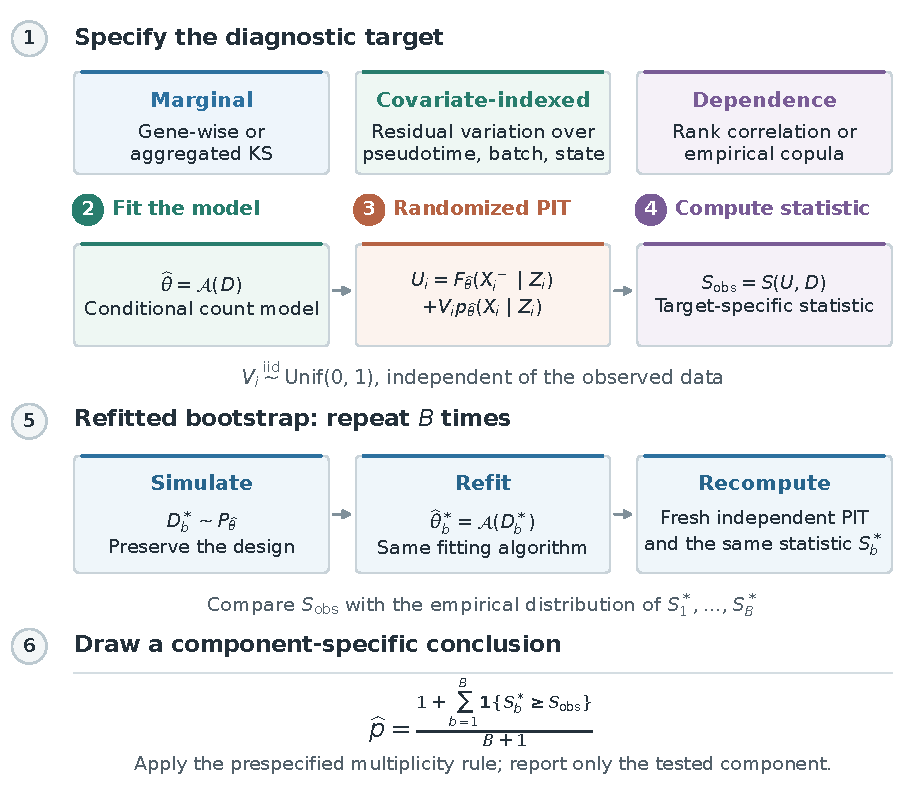
\includegraphics[width=\linewidth]{figs/calibration_workflow_revised.pdf}
\caption{Randomized-PIT diagnostic workflow for a fitted model. Data $D$
contain counts $X$ and covariates $Z$; $\mathcal A$ is the fitting algorithm.
The chosen target determines the statistic: separate marginal KS statistics
do not test dependence. Bootstrap calibration repeats the same fitting and
diagnostic operations, including fresh residual randomization. If the null
is fully specified, the appropriate fixed-null law replaces steps 2 and 5,
provided its sampling conditions hold. Fitted-model bootstrap validity
requires the regularity and consistency conditions stated in Section 3.}
\label{fig:article-map}
\end{figure}

The plus-one rule avoids reporting zero Monte Carlo $p$-values; its resolution
is $1/(B+1)$. It does not make a fitted parametric bootstrap finite-sample
exact. Its inferential justification depends on the model, sampling design,
and bootstrap conditions stated in Section~\ref{sec:theory}. A small
$p$-value flags a discrepancy in the tested component; a large value does
not establish that the component, or the full simulator, is correct.

\begin{table}[!htbp]
\centering
\scriptsize
\caption{Diagnostic targets, reference laws, and the conclusions supported by
the workflow.}
\label{tab:diagnostic-targets}
\setlength{\tabcolsep}{3pt}
\begin{tabular}{@{}>{\raggedright\arraybackslash}p{0.15\linewidth}>{\raggedright\arraybackslash}p{0.20\linewidth}>{\raggedright\arraybackslash}p{0.20\linewidth}>{\raggedright\arraybackslash}p{0.19\linewidth}>{\raggedright\arraybackslash}p{0.18\linewidth}@{}}
\toprule
Target & Example statistic & Reference & Supported conclusion & Not established\\
\midrule
Marginal count fit & Gene-wise or aggregated uniform KS & Fixed law for known margins; refitted bootstrap for fitted margins & Evidence of discrepancies in the specified marginal count distributions & Gene--gene dependence or covariate structure\\
\addlinespace
Conditional fit & Residual process indexed by pseudotime, batch, or cell state & Refitted bootstrap preserving the conditioning design & Evidence of residual variation over the indexed covariate & Unindexed dependence components\\
\addlinespace
Dependence fit & Residual rank correlation, empirical copula, or Rosenblatt statistic & Joint fitted-model simulation with refitting & Evidence of discrepancies in the tested dependence feature & All higher-order dependence unless included in the statistic\\
\bottomrule
\end{tabular}
\end{table}

\section{Theoretical Justification}\label{sec:theory}

\subsection{Fixed-null baseline}\label{sec:fixed-null}

The classical finite-sample KS reference law applies to independent uniforms
under a fully specified null. On the uniform scale, the one-sample
empirical path drifts between observations and jumps at observations; exact
one-sided and two-sample probabilities can therefore be written as finite
crossing or path-counting calculations. These fixed-null formulas are the
baseline against which fitted-simulator diagnostics should be judged. The
detailed crossing formulas, recursions, and limiting fixed-null identities are
given in Supplementary Appendix A--D.

The point needed for single-cell simulators is simple. If a known count margin
is applied to independent draws and transformed by the randomized probability
integral transform, the transformed residuals are independent uniforms and the
ordinary KS crossing law applies. If the same margin is estimated first, the
residual path is no longer the fixed-null empirical bridge. The fitting step
must be included in the
reference law, either analytically through a fitted empirical-process limit or
computationally through a refitted bootstrap. We state this fitted-null
principle first for ordinary composite models and then specialize it to
randomized residuals for scDesign-style count simulators.

\subsection{Composite nulls and parameter estimation}
\label{sec:composite}
Everything in the fixed-null argument relies on knowing the null distribution
before seeing the data. Once parameters are estimated from the same data, the
transformed observations no longer behave like independent uniforms under a
fixed distribution. The path being tested has been altered by the fitting
step, so the ordinary distribution-free calibration no longer applies.

Let $X_1,\ldots,X_n$ be independent observations from $F_\theta$, with
unknown parameter vector $\theta$. For a normal distribution,
$\theta=(\mu,\sigma^2)^T$. Estimate $\theta$ by maximum likelihood or
another regular method, and define
\begin{align}
    Z_n(t,\theta)&=\sqrt{n}\left(F_n(t)-F_\theta(t)\right)\\
    Z_n(t,\widehat{\theta})&=\sqrt{n}\left(F_n(t)-F_{\widehat{\theta}}(t)\right).
\end{align}
The key step in classical composite-null KS theory is a first-order expansion
of the fitted distribution
\citep{durbin1973weak,babu2004goodness,van2000asymptotic,del2007lectures}:
\begin{align*}
    Z_n(t,\widehat{\theta})&=Z_n(t,\theta)+\sqrt{n}\left(F_\theta(t)-F_{\widehat{\theta}}(t)\right)\\
    &=Z_n(t,\theta)-\frac{\partial F_\theta(t)}{\partial\theta}^T\sqrt{n}(\widehat{\theta}-\theta)+o_{\mathbb{P}_\theta}(1)\\
    &=Z_n(t,\theta)-\frac{\partial F_\theta(t)}{\partial\theta}^T\frac{1}{\sqrt{n}}\sum_{i=1}^n\psi_\theta(X_i)+o_{\mathbb{P}_\theta}(1)
\end{align*}
Here the estimator is assumed to admit the expansion
\[
\sqrt{n}(\widehat{\theta}-\theta)=\frac{1}{\sqrt{n}}\sum_{i=1}^n\psi_\theta(X_i)+o_{\mathbb{P}_\theta}(1),
\]
The influence function $\psi_\theta$ describes each observation's
first-order contribution to the estimator and has mean zero and finite
second moment. The fitted-process limit follows from the joint limit of
\[
\left(Z_n(\cdot,\theta),\frac{1}{\sqrt{n}}\sum_{i=1}^n\psi_\theta(X_i)\right).
\]
Donsker's theorem gives $Z_n(\cdot,\theta)\Rightarrow B(F_\theta(\cdot))=B\circ F_\theta$, where $B$ is a standard Brownian bridge, while the central limit theorem gives $\frac{1}{\sqrt{n}}\sum_{i=1}^n\psi_\theta(X_i)\Rightarrow \mathcal{N}(0,\Sigma(\theta))$, where $\Sigma(\theta)=\mathbb{E}\psi_\theta(X_1)^{\otimes 2}$. The covariance can be computed from
\[
\Cov(\mathbb{I}(X_1\le t),\psi_\theta(X_1))=\int_{-\infty}^t\psi_\theta(x)F_\theta(dx):=h(t,\theta).
\]
Hence, we have finite-dimensional weak convergence. Tightness then yields weak convergence of the stochastic process $Z_n(t,\widehat{\theta})$ \citep{babu2004goodness}; the limit is a mean-zero Gaussian process $Z(\cdot,\theta)$ with covariance
\begin{align}\label{eq:cov}
    \Cov\left(Z(s,\theta),Z(t,\theta)\right)
    &=F_\theta(s\wedge t)-F_\theta(s)F_\theta(t)\\
    &\quad-h(t,\theta)^T\frac{\partial F_\theta(s)}{\partial \theta}\nonumber\\
    &\quad-h(s,\theta)^T\frac{\partial F_\theta(t)}{\partial \theta}\nonumber\\
    &\quad+\frac{\partial F_\theta(s)}{\partial\theta}^T
      \Sigma(\theta)
      \frac{\partial F_\theta(t)}{\partial\theta}.\nonumber
\end{align}

The following theorem states the conditions needed for this expansion.
\begin{theorem}[Durbin-Babu-Rao \citep{durbin1973weak,babu2004goodness}]
Let $X_1,\ldots,X_n$ be a random sample with common distribution function
$F_\theta$ and $\theta\in\mathbb{R}^k$. Let $\widehat{\theta}$ be an estimator
of $\theta$ with influence function $\psi_\theta$. Assume that
\[
\sqrt n(\widehat\theta-\theta)
=n^{-1/2}\sum_{i=1}^n\psi_\theta(X_i)+o_{\mathbb P_\theta}(1),
\]
that $F_\theta(t)$ is uniformly differentiable in $\theta$ along
$\widehat\theta-\theta$, so that
\[
\sup_t\left|
\sqrt n\{F_{\widehat\theta}(t)-F_\theta(t)\}
-\frac{\partial F_\theta(t)}{\partial\theta}^T
\sqrt n(\widehat\theta-\theta)
\right|=o_{\mathbb P_\theta}(1),
\]
and that, with $P_n$ denoting the empirical measure and $P_\theta$ the law
under $F_\theta$, the empirical process and estimator expansion converge
jointly,
\[
\left(\sqrt n(P_n-P_\theta)\mathbf 1\{X\le \cdot\},
n^{-1/2}\sum_{i=1}^n\psi_\theta(X_i)\right)
\Rightarrow (B_\theta,Z_\theta)
\]
in $\ell^\infty(\mathcal T)\times\mathbb R^k$, where $\mathcal T$ is the index
set over which the KS supremum is taken. Define
\[
\Sigma(\theta)=\mathbb E_\theta\{\psi_\theta(X)\psi_\theta(X)^T\},
\qquad
h(t,\theta)=\mathbb E_\theta[\{\mathbf 1(X\le t)-F_\theta(t)\}\psi_\theta(X)].
\]
Assume the joint limit has cross-covariance
$\Cov\{B_\theta(t),Z_\theta\}=h(t,\theta)$, and define
\[
D_n(\widehat{\theta})=\sup_{t}|F_n(t)-F_{\widehat{\theta}}(t)|.
\]
Then, at every continuity point $\epsilon$ of the limiting law,
\[
\mathbb{P}\left(\sqrt{n}D_n(\widehat{\theta})>\epsilon\right)
\longrightarrow
\mathbb{P}\left(\sup_t|Z(t,\theta)|>\epsilon\right),
\]
where
\[
Z(t,\theta)=B_\theta(t)
-\frac{\partial F_\theta(t)}{\partial\theta}^T Z_\theta
\]
is a mean-zero Gaussian process with covariance specified in \eqref{eq:cov}.
Bootstrap or Monte Carlo approximations require the corresponding consistency
conditions for this fitted-null process.
\end{theorem}

\noindent\textit{Proof.} This is the classical composite-null expansion; a
derivation in the notation used here is given in Supplementary Appendix F.

\begin{remark}[Consequences of naive KS calibration]
If one estimates the parameter and then
uses the classical Brownian-bridge critical value as if $\theta$ were known, the
test uses an inappropriate reference law. Table~\ref{tab:composite-null}
illustrates the resulting conservatism at nominal level $5\%$ with $n=100$.
The classical cutoff is
$1.358/\sqrt{n}$; the bootstrap column uses a parametric bootstrap in which
parameters are re-estimated in every bootstrap sample. Implementation details
are given in Supplementary Appendix H.
\end{remark}

\begin{table}[!htbp]
\centering
\small
\caption{Empirical rejection probabilities under the null, based on 2000 Monte
Carlo samples. The bootstrap column uses 399 bootstrap resamples per Monte Carlo
sample.}
\label{tab:composite-null}
\begin{tabular}{@{}lcc@{}}
\toprule
Null model & KS cutoff & Refit bootstrap\\
\midrule
Known $N(0,1)$ & 0.051 & --\\
Fitted normal $(\mu,\sigma^2)$ & 0.000 & 0.044\\
Fitted exponential rate & 0.007 & 0.052\\
\bottomrule
\end{tabular}
\end{table}

\begin{remark}[Cases outside the linear expansion]
There are also models where the Durbin-Babu-Rao expansion itself should not be
used without extra work. A simple example is a distribution with parameter-dependent
support, such as $\operatorname{Unif}(0,\theta)$ with $\theta$
estimated by the sample maximum: the estimator has an $n$-rate, non-Gaussian
limit and is not asymptotically linear in the form assumed above. Mixture
models near nonidentifiable parameter values create a different version of the
same problem. In such cases, a refitted simulation scheme may still be useful,
but the limiting Gaussian projection in \eqref{eq:cov} is no longer the right
justification.
\end{remark}

\begin{remark}
In the case of maximum likelihood estimation, the influence function is
\[
\psi_\theta(x)=I^{-1}_\theta s_\theta(x),
\]
where $I^{-1}_\theta$ is the inverse of Fisher information and $s_\theta(x)$ is the score function evaluated at $x$.
\end{remark}


\begin{example}
Let $X\sim N(\mu,\sigma^2)$. The influence function for the maximum likelihood estimator is
\[
\psi_\theta(x)=
\begin{pmatrix}
    x-\mu\\
    (x-\mu)^2-\sigma^2
\end{pmatrix},
\]
and
\[
\Sigma(\theta)=I_\theta^{-1}=
\begin{pmatrix}
    \sigma^2 & 0\\
    0 & 2\sigma^{4}
\end{pmatrix}.
\]
\end{example}

\subsection{Randomized residual processes for fitted discrete models}
\label{sec:scdesign}

Single-cell trend models and count simulators add one more layer to the
fitted-null problem. Counts are discrete, so the ordinary probability integral
transform is not uniform without randomization. Moreover, trend and simulator
parameters are fitted before the diagnostic is computed. This section gives
the resulting calibration rules for fitted count margins, including
scGTM-style conditional trends and scDesign-style margins and copulas.
The conditions below have three practical roles: the estimator must have a
stable first-order approximation, the residual distribution must vary smoothly
with the fitted parameter, and the empirical fluctuation must remain controlled
when that parameter is substituted. A Donsker condition is one way to obtain
a Gaussian approximation uniformly over residual thresholds. These properties
must be checked for the chosen model and fitting procedure.

\begin{theorem}[Residual empirical-process calibration]
\label{thm:residual-crossing-principle}
Let $(X_i,W_i)$ be independent copies of $(X,W)$, where $W$ is an auxiliary
randomizer independent of $X$. The estimator is computed from the observed
$X_i$'s before the auxiliary randomizers are generated. Let
$\{T_\theta:\theta\in\Theta\}$ be measurable maps from the data-randomizer
space into $(0,1)$, and suppose that
$T_{\theta_0}(X,W)\sim\operatorname{Unif}(0,1)$. Write $P_n$ for the empirical
measure of $(X_i,W_i)$ and $P_{\theta_0}$ for the law of $(X,W)$ at the true
parameter. Let $\widehat\theta$ satisfy
\[
\sqrt n(\widehat\theta-\theta_0)
=\frac{1}{\sqrt n}\sum_{i=1}^n\psi_{\theta_0}(X_i)+o_{\mathbb P}(1).
\]
Define
\[
\begin{aligned}
H_\theta(u)
&=\Prob_{\theta_0}\{T_\theta(X,W)\le u\},\\
\alpha_n(u)
&=\sqrt n\left\{\frac{1}{n}\sum_{i=1}^n
\mathbf 1\{T_{\widehat\theta}(X_i,W_i)\le u\}-u\right\}.
\end{aligned}
\]
Assume:
\begin{enumerate}
\item the class $\{\mathbf 1(T_{\theta_0}\le u):0<u<1\}$ is Donsker;
\item the local plug-in empirical-process remainder satisfies
\[
\sup_{0<u<1}\sqrt n\left|
(P_n-P_{\theta_0})\{\mathbf 1(T_{\widehat\theta}\le u)
-\mathbf 1(T_{\theta_0}\le u)\}\right|=o_{\mathbb P}(1);
\]
\item the deterministic centering map is locally uniformly linear along
$\widehat\theta$, namely
\[
\sup_{0<u<1}\left|
\sqrt n\{H_{\widehat\theta}(u)-H_{\theta_0}(u)\}
-\dot H_{\theta_0}(u)^T\sqrt n(\widehat\theta-\theta_0)
\right|=o_{\mathbb P}(1);
\]
\item the process
$\sqrt n(P_n-P_{\theta_0})\mathbf 1\{T_{\theta_0}\le u\}$ in
$\ell^\infty(0,1)$ and $\sqrt n(\widehat\theta-\theta_0)$ converge jointly to
$(B,Z_\theta)$.
\end{enumerate}
Then in $\ell^\infty(0,1)$,
\[
\alpha_n(u)\Rightarrow B(u)+\dot H_{\theta_0}(u)^T Z_\theta,
\]
where $B$ is a Brownian bridge and $Z_\theta$ is the Gaussian limit of
$\sqrt n(\widehat\theta-\theta_0)$, jointly distributed with $B$.
Consequently, if
\[
K_n=\sup_{0<u<1}|\alpha_n(u)|,
\]
then at continuity points $c$ of the law of
$\sup_{0<u<1}|B(u)+\dot H_{\theta_0}(u)^T Z_\theta|$,
\[
\mathbb P(K_n\le c)\to
\mathbb P\left\{\sup_{0<u<1}|B(u)+\dot H_{\theta_0}(u)^T Z_\theta|\le c\right\}.
\]
\end{theorem}

\begin{proof}
For the random $\widehat\theta$, $H_{\widehat\theta}(u)$ means the deterministic map
$\theta\mapsto H_\theta(u)$ evaluated at $\widehat\theta$. Add and subtract the
process at the true parameter:
\[
\alpha_n(u)
=\sqrt n(P_n-P_{\theta_0})\mathbf 1\{T_{\theta_0}\le u\}
+R_n(u)+\sqrt n\{H_{\widehat\theta}(u)-u\},
\]
where
\[
R_n(u)=\sqrt n(P_n-P_{\theta_0})
\{\mathbf 1(T_{\widehat\theta}\le u)-\mathbf 1(T_{\theta_0}\le u)\}.
\]
The first term converges to a Brownian bridge because
$T_{\theta_0}(X,W)$ is uniform and the indicator class is Donsker. Assumption 2
gives $\sup_u|R_n(u)|=o_{\mathbb P}(1)$. Since
$H_{\theta_0}(u)=u$, Assumption 3 gives the uniformly valid expansion
\[
\sqrt n\{H_{\widehat\theta}(u)-u\}
=\dot H_{\theta_0}(u)^T\sqrt n(\widehat\theta-\theta_0)+o_{\mathbb P}(1)
\]
in $\ell^\infty(0,1)$. The joint convergence in Assumption 4 completes the
proof.
\end{proof}

This theorem applies the classical expansion to a specified residual map; it
does not verify regularity for a particular simulator. The map $T_\theta$ may be a randomized
PIT for a count simulator, a Rosenblatt-type transform for a copula, or a
residual transform for a fitted conditional count model, once the listed
empirical-process conditions have been verified for that transform. The
local plug-in remainder in Assumption 2 is the substantive condition: it is
where one verifies that estimating $\theta$ does not add an unaccounted
indicator-class fluctuation beyond the displayed derivative term. In smooth
finite-dimensional settings with fixed support this is typically proved from
stochastic equicontinuity of the threshold class and root-$n$ consistency of
the estimator. For penalized, black-box, nonregular, clustered, or
high-dimensional simulator fits, this condition is not automatic. Repeating the
fitting algorithm in a bootstrap does not establish it or prove bootstrap
consistency. When the required conditions have not been verified, the
refitted reference is an empirical approximation whose accuracy needs a
model-specific assessment. The ordinary KS law is recovered in the
fixed-parameter case, and in fitted cases only under additional degeneracy or
cancellation, for example a vanishing first-order derivative term.

For an integer-valued distribution function $F$, write
$F(k-)=\Prob(X<k)$ and $p_F(k)=F(k)-F(k-)$. For $v\in(0,1)$ define the
randomized distributional transform
\[
T_F(k,v)=F(k-)+v\,p_F(k).
\]
This is the form of the randomized transform used for discrete margins in the
scDesign2 copula construction, up to the equivalent convention for the
uniform randomizer \citep{sun2021scdesign2,sun2023scdesign2correction}.

\begin{proposition}[Exact marginal crossings for known discrete margins]
\label{prop:known-discrete-margin}
Let $X_1,\ldots,X_n$ be independent observations from a known integer-valued
count distribution $F$ on a countable ordered support, and let
$V_1,\ldots,V_n$ be independent $\operatorname{Unif}(0,1)$ variables
independent of the counts. Set $U_i=T_F(X_i,V_i)$. The resulting variables are
independent and each has the $\operatorname{Unif}(0,1)$ law. Consequently their
KS statistics have the ordinary simple-null uniform-scale calibration; in
particular, the one-sided statistic has the fixed-null crossing law summarized
in Section~\ref{sec:fixed-null} and detailed in the supplementary appendix.
\end{proposition}

\begin{proof}
Conditional on $X_i=k$, $U_i$ is uniform on the interval
$(F(k-),F(k)]$. The intervals with $p_F(k)>0$ partition $(0,1)$ up to endpoints and
have lengths $p_F(k)$. For any $u\in(0,1)$, choose a count $k$ with
$p_F(k)>0$ and $F(k-)\le u\le F(k)$; at shared endpoints either adjacent
positive-mass interval gives the same value. Then
\[
\begin{aligned}
\Prob(U_i\le u)
&=\sum_{\ell<k}p_F(\ell)+p_F(k)
  \Prob\{F(k-)+V_i p_F(k)\le u\mid X_i=k\}\\
&=F(k-)+u-F(k-)=u.
\end{aligned}
\]
Thus each $U_i$ is uniform on $(0,1)$. Independence follows because the pairs
$(X_i,V_i)$ are independent. The exact KS crossing formulas then apply to the
transformed sample.
\end{proof}

The preceding proposition is exact but it assumes that the margin is known.
Fitted single-cell simulators do not have this property. The next result is the
discrete residual analogue of the fitted-null empirical-process calculation in
Section~\ref{sec:composite}.

\begin{corollary}[Plug-in randomized bridge under regular fitted margins]
\label{thm:randomized-plugin-bridge}
Let $\{F_\theta:\theta\in\Theta\subset\mathbb{R}^q\}$ be a parametric family
of discrete count distributions and suppose the data are generated from
$F_{\theta_0}$. Let $\widehat\theta$ be an estimator satisfying
\[
\sqrt n(\widehat\theta-\theta_0)
=\frac{1}{\sqrt n}\sum_{i=1}^n\psi_{\theta_0}(X_i)+o_{\mathbb P}(1).
\]
For independent $V_i\sim\operatorname{Unif}(0,1)$, define
$U_i(\theta)=T_{F_\theta}(X_i,V_i)$ and
\[
\alpha_n(u)=
\sqrt n\left\{
\frac{1}{n}\sum_{i=1}^n\mathbf 1\{U_i(\widehat\theta)\le u\}-u
\right\},\qquad 0<u<1.
\]
Let
\[
G_\theta(u)=\Prob_{\theta_0}\{T_{F_\theta}(X,V)\le u\}
\]
and assume that the four conditions in
Theorem~\ref{thm:residual-crossing-principle} hold for this transform, with
$H_\theta=G_\theta$. In particular, this assumes that the local plug-in
empirical-process remainder is negligible and that the deterministic centering
map is locally uniformly linear along $\widehat\theta$, with derivative
$\dot G_{\theta_0}(u)$. Then in
$\ell^\infty(0,1)$,
\[
\alpha_n(u)\Rightarrow B(u)+\dot G_{\theta_0}(u)^T Z_\theta,
\]
where $B$ is a Brownian bridge and $Z_\theta$ is the Gaussian limit of
$\sqrt n(\widehat\theta-\theta_0)$, jointly distributed with $B$.
\end{corollary}

\noindent\textit{Proof.} Substitute the randomized discrete transform into
Theorem~\ref{thm:residual-crossing-principle}; details are given in
Supplementary Appendix F.

\begin{corollary}[Refitted simulator bootstrap under conditional expansion]
\label{cor:refitted-bootstrap}
Assume the conditions of Corollary~\ref{thm:randomized-plugin-bridge} and,
conditional on the observed data, the bootstrap analogues of the Donsker/tightness
condition, local plug-in remainder, local centering linearity, asymptotic
linearity, and joint convergence conditions. More explicitly, assume also that
$\widehat\theta\to_{\mathbb P}\theta_0$, that the conditional joint law of the
bootstrap empirical process and
$\sqrt n(\widehat\theta^*-\widehat\theta)$ converges in probability to the same
Gaussian pair $(B,Z_\theta)$ as in
Corollary~\ref{thm:randomized-plugin-bridge}, and that the derivative
$\dot G_{\widehat\theta}^*(u)$ of the conditional bootstrap centering map
satisfies
\[
\sup_{0<u<1}\|\dot G_{\widehat\theta}^*(u)-\dot G_{\theta_0}(u)\|
\to_{\mathbb P}0 .
\]
Conditional on the observed data $\mathcal D_n$, generate
\[
X_i^*\stackrel{\mathrm{ind}}{\sim}F_{\widehat\theta},\qquad
V_i^*\stackrel{\mathrm{ind}}{\sim}\operatorname{Unif}(0,1),
\qquad i=1,\ldots,n,
\]
with the bootstrap counts and uniforms conditionally independent. Refit the
parameter to obtain $\widehat\theta^*$ and compute
\[
K_n^*=\sup_{0<u<1}
\left|
\sqrt n\left\{\frac{1}{n}\sum_{i=1}^n
\mathbf 1\{T_{F_{\widehat\theta^*}}(X_i^*,V_i^*)\le u\}-u\right\}
\right|.
\]
Then the conditional distribution of $K_n^*$ consistently estimates the
limiting distribution of $K_n=\sup_{0<u<1}|\alpha_n(u)|$: for every continuity
point $c$ of the limiting law,
\[
\mathbb P^*(K_n^*\le c\mid\mathcal D_n)
-
\mathbb P(K_n\le c)
\to_{\mathbb P}0 .
\]
If the bootstrap sample is generated from $F_{\widehat\theta}$ but the
parameter is held fixed when the statistic is recomputed, the bootstrap
calibrates the process obtained by holding that fitted margin fixed, rather
than the complete fitted workflow. It omits the first-order estimation term except in degenerate
cases where that term vanishes.
\end{corollary}

\noindent\textit{Proof.} Apply the residual-process expansion conditionally
under the bootstrap law. The full conditional expansion is given in
Supplementary Appendix F.

\begin{proposition}[A marginal KS blind spot for copula simulators]
\label{prop:copula-blind-spot}
Consider independent cells from a scDesign2-style simulator with fixed margins
$F_1,\ldots,F_p$ and copula parameter $R$. Let $R'$ be another copula
parameter with the same margins. For any fixed gene $j$, the randomized
residuals
\[
U_{ij}=T_{F_j}(X_{ij},V_{ij}),\qquad i=1,\ldots,n,
\]
have the same marginal distribution under $R$ and $R'$. Hence any diagnostic
or rejection rule measurable only with respect to the empirical distribution of
$U_{1j},\ldots,U_{nj}$ has the same rejection probability under $R$ and $R'$;
it has no power beyond its size against alternatives that change only the
dependence structure. This statement does not cover procedures that use the
joint law of multiple gene-wise residual processes across paired cells.
\end{proposition}

\begin{proof}
A copula changes the joint distribution within a cell while preserving all
univariate margins. Proposition~\ref{prop:known-discrete-margin} converts the
$j$th margin to uniform residuals regardless of the copula parameter, and the
cells are independent by assumption. This is only a statement about a fixed
gene's marginal residual process; it does not assert cross-gene independence.
Therefore a single-gene KS process has the same distribution under $R$ and
$R'$. Across cells, independence makes the empirical distribution a sample from
the same univariate uniform law under both copulas. This proves only a
single-gene marginal statement, not a claim about diagnostics that combine
paired residuals across genes.
\end{proof}

\begin{remark}
Proposition~\ref{prop:copula-blind-spot} does not say that copula
misspecification is invisible. It says that it is invisible to a single-gene
marginal KS diagnostic. Dependence diagnostics must use joint residual
structure, for example pairwise residual ranks, empirical copula processes, or
two-dimensional crossing statistics on $(U_j,U_k)$.
\end{remark}

\begin{remark}[Conditional residual diagnostics]
\label{rem:conditional-residuals}
Let $Z_i$ denote a cell-level covariate such as cell type, pseudotime, batch,
modality, or spatial location. This includes pseudotime trend models such as
scGTM and conditional simulator margins such as those fitted by scDesign3
\citep{cui2022scgtm,song2024scdesign3}. Condition on the observed covariates,
or assume independent cells with covariates $Z_i$. If a known conditional
count margin $F_{\theta_0}(\cdot\mid Z_i)$ is correctly specified, then
\[
U_i=T_{F_{\theta_0}(\cdot\mid Z_i)}(X_i,V_i)
\]
satisfies $U_i\mid Z_i\sim\operatorname{Unif}(0,1)$, and the residuals are
conditionally independent when the cells are. Thus residual non-uniformity
within covariate regions, or residual association between $U_i$ and $Z_i$, is a
population lack-of-fit signal; after fitting, it is descriptive unless
calibrated by the fitted conditional workflow.
The statement treats $Z_i$ as fixed or external to the count-margin fit. If
pseudotime, cell type, batch labels, or other covariates are estimated from the
same expression data, that estimation step becomes part of the fitted workflow
and must be included in the empirical-process expansion or in the refitted
bootstrap.

With fitted conditional parameters, the analogous residual process is a
plug-in empirical process indexed by both the residual threshold and the
covariate region. A formal version requires indexed empirical-process
conditions of the same type as above, such as a manageable covariate class,
local centering linearity of the conditional margin, and a joint limit for the
fitted conditional parameter.
Accordingly, simple uniform KS summaries are descriptive unless they are
calibrated by the fitted conditional workflow, for example by a refitted
bootstrap.
\end{remark}

\section{Interpretation for Fitted Simulator Diagnostics}\label{sec:interpretation}

The fitted-null limit can be read geometrically for efficient estimation in
regular parametric models:
fitting removes empirical-process variation in score directions, so the
residual bridge is a plug-in or projected Gaussian process rather than the
ordinary Brownian bridge. This interpretation is useful, but it is not needed
to run the diagnostic. In practice, the operational requirement is to calibrate
the exact statistic generated by the fitted simulator workflow, including the
same estimation, randomization, and residual transformation steps used on the
observed data. Supplementary Appendix E gives the geometric and finite
crossing-complex interpretation.

\section{Simulation Studies and Real-Data Diagnostics}
\label{sec:simulation-studies}

\subsection{Simulation Studies}
\label{sec:simulations}

We evaluate the effect of parameter estimation on randomized-PIT KS tests
using independent negative-binomial counts with mean $6$, size parameter
$r=2.5$, and variance $6+6^2/r$. At $n=250$, 1,000, and 10,000, we compare
four reference procedures: the ordinary KS cutoff with known parameters,
the same cutoff after moment fitting, a fixed-parameter bootstrap, and a
refitted bootstrap. The nominal level is $5\%$. Power is assessed by adding a
15\% point mass at zero to the generating distribution. Separate experiments
examine conditional-mean and copula misspecification. Supplementary Appendix H
gives the estimation rules and implementation details.

\begin{table}[!htbp]
\centering
\scriptsize
\caption{Negative-binomial randomized residual calibration across sample
sizes. The null Monte Carlo sample sizes are 400, 250, and 300, and the
corresponding bootstrap sizes are 199, 149, and 99. Power is evaluated against
a negative-binomial distribution mixed with a 15\% point mass at zero using 200, 125,
and 100 Monte Carlo samples. ``Fixed boot'' simulates from the fitted model but
does not refit it; ``refit boot'' repeats parameter estimation. The four
type-I error columns are empirical null rejection proportions at nominal
level 0.05. Power is the refitted-bootstrap rejection proportion under the
zero-inflated alternative.}
\label{tab:nb-scale}
\setlength{\tabcolsep}{3pt}
\begin{tabular}{@{}rcccccc@{}}
\toprule
 & \multicolumn{4}{c}{Empirical type-I error} & & \\
\cmidrule{2-5}
$n$ & Known & Naive KS & Fixed boot & Refit boot & Refit power & Runtime (s)\\
\midrule
250 & 0.052 & 0.000 & 0.000 & 0.062 & 0.955 & 13.5\\
1,000 & 0.056 & 0.000 & 0.000 & 0.040 & 1.000 & 12.9\\
10,000 & 0.047 & 0.000 & 0.003 & 0.040 & 1.000 & 68.4\\
\bottomrule
\end{tabular}
\end{table}

Across the three sample sizes, the ordinary KS cutoff after fitting yields
no rejections, and the fixed-parameter bootstrap yields rejection rates of
0.0--0.3\% (Table~\ref{tab:nb-scale}). Refitting yields rejection rates of
4.0--6.2\%, close to the nominal 5\%, with power of 95.5--100\% against the
zero-inflated alternative. These results show that parameter re-estimation,
not simulation alone, is needed to reproduce the null variation of the fitted
residual statistic in this setting.

The estimation effect need not disappear from the reference law as $n$
increases. Although $\widehat\theta-\theta_0=O_{\mathbb P}(n^{-1/2})$,
the KS process is also multiplied by $\sqrt n$. Its estimation term therefore
remains $O_{\mathbb P}(1)$:
\[
\alpha_n(u)=B_n(u)+\dot G_{\theta_0}(u)^T
\sqrt n(\widehat\theta-\theta_0)+o_{\mathbb P}(1),
\]
where $B_n$ denotes the empirical process at the true margin. The unscaled
discrepancy shrinks, but the difference between fixed-null and fitted-null
critical values can persist on the scale used for testing. The rejection
rates in Table~\ref{tab:nb-scale} illustrate this distinction; their Monte
Carlo uncertainty is reported in Supplementary Appendix H.

\begin{table}[!htbp]
\centering
\scriptsize
\caption{Component-specific simulations. Panel A uses two independent
240-cell samples per trial, known NB margins, and 1000 trials; brackets are
95\% Wilson intervals. Panel B uses scDesign3 NB regressions, 500 outer
samples per scenario, and 199 bootstrap refits per sample; brackets are
exact 95\% binomial intervals. The conditional statistic is the maximum
of all six scaled between-quartile KS distances. ``Fixed'' omits refitting;
``refit'' repeats the complete fit and statistic. The two diagnostic
targets are reported separately, not combined into one rejection rule.
The Periodic / linear row reports power; the other Panel B rows report size.}
\label{tab:scdesign-simulations}
\begin{tabular}{@{}lccc@{}}
\toprule
\multicolumn{4}{@{}l}{A. Copula misspecification with known margins}\\
Scenario & Gene 1 KS & Gene 2 KS & Correlation\\
\midrule
Same ($\rho=0.65$) & 0.043 [0.032;0.057] & 0.052 [0.040;0.068] & 0.058 [0.045;0.074]\\
Wrong ($\rho=0.50$) & 0.054 [0.042;0.070] & 0.050 [0.038;0.065] & 0.663 [0.633;0.692]\\
Independent ($\rho=0$) & 0.039 [0.029;0.053] & 0.049 [0.037;0.064] & 1.000 [0.996;1.000]\\
\bottomrule
\end{tabular}
\par\medskip
\begin{tabular}{@{}lcccc@{}}
\toprule
\multicolumn{5}{@{}l}{B. Fitted conditional margins: generating / fitted mean}\\
Scenario & $n$ & Marginal refit & Conditional fixed & Conditional refit\\
\midrule
\inputresultrows{results/conditional_calibration/main_table_rows.tex}
\bottomrule
\end{tabular}
\end{table}

The copula block implements Proposition~\ref{prop:copula-blind-spot}. Samples
are generated from two negative-binomial margins joined by a Gaussian copula
with data-generating correlation $\rho=0.65$. When the synthetic sample uses the
wrong copula correlation but the same margins, including the moderate
$\rho=0.50$ change and the stronger $\rho=0$ independence misspecification,
the two gene-wise marginal KS diagnostics remain near the nominal level. A
residual correlation diagnostic, however, reacts to dependence
misspecification, with partial power for the moderate change and near-certain
power for the independence case. The correlation reference is approximate;
this known-margin experiment is not a test of fitted copula calibration.

Panel B evaluates the complete conditional-margin procedure using
scDesign3's NB regression function. On fixed pseudotimes, we simulate
log-linear, periodic, and cubic-spline mean curves and re-estimate both
the mean and NB size in every bootstrap sample, including smoothing for
the spline fit. The two statistics are the marginal KS and the maximum
of six scaled between-quartile KS distances. Each maximum is calibrated
as one statistic; six unadjusted pairwise tests are not used.
The sample size is 240 for the linear and periodic models and 2,087 for
the spline null, whose fitting configuration matches the pancreatic
conditional margins. Supplementary Appendix H.5 specifies the generating
curves, fitting rules, and independent observed and bootstrap streams.
Across the three correctly specified cases, refitted marginal rejection
rates range from 4.8\% to 6.4\%, and
conditional rejection rates from 5.2\% to 6.4\%.
When the periodic component is omitted, conditional rejection is
92.4\%, compared with 8.4\% for the marginal statistic.
The two diagnostic targets thus have different sensitivity to the
omitted trend in this setting. These are finite-sample
checks of the specified regressions, with Monte Carlo uncertainty shown
in the table, not a proof of validity for arbitrary fitted simulators.
All 398,000 bootstrap refits and 2,000 observed fits succeeded.


\begin{figure}[t]
\centering
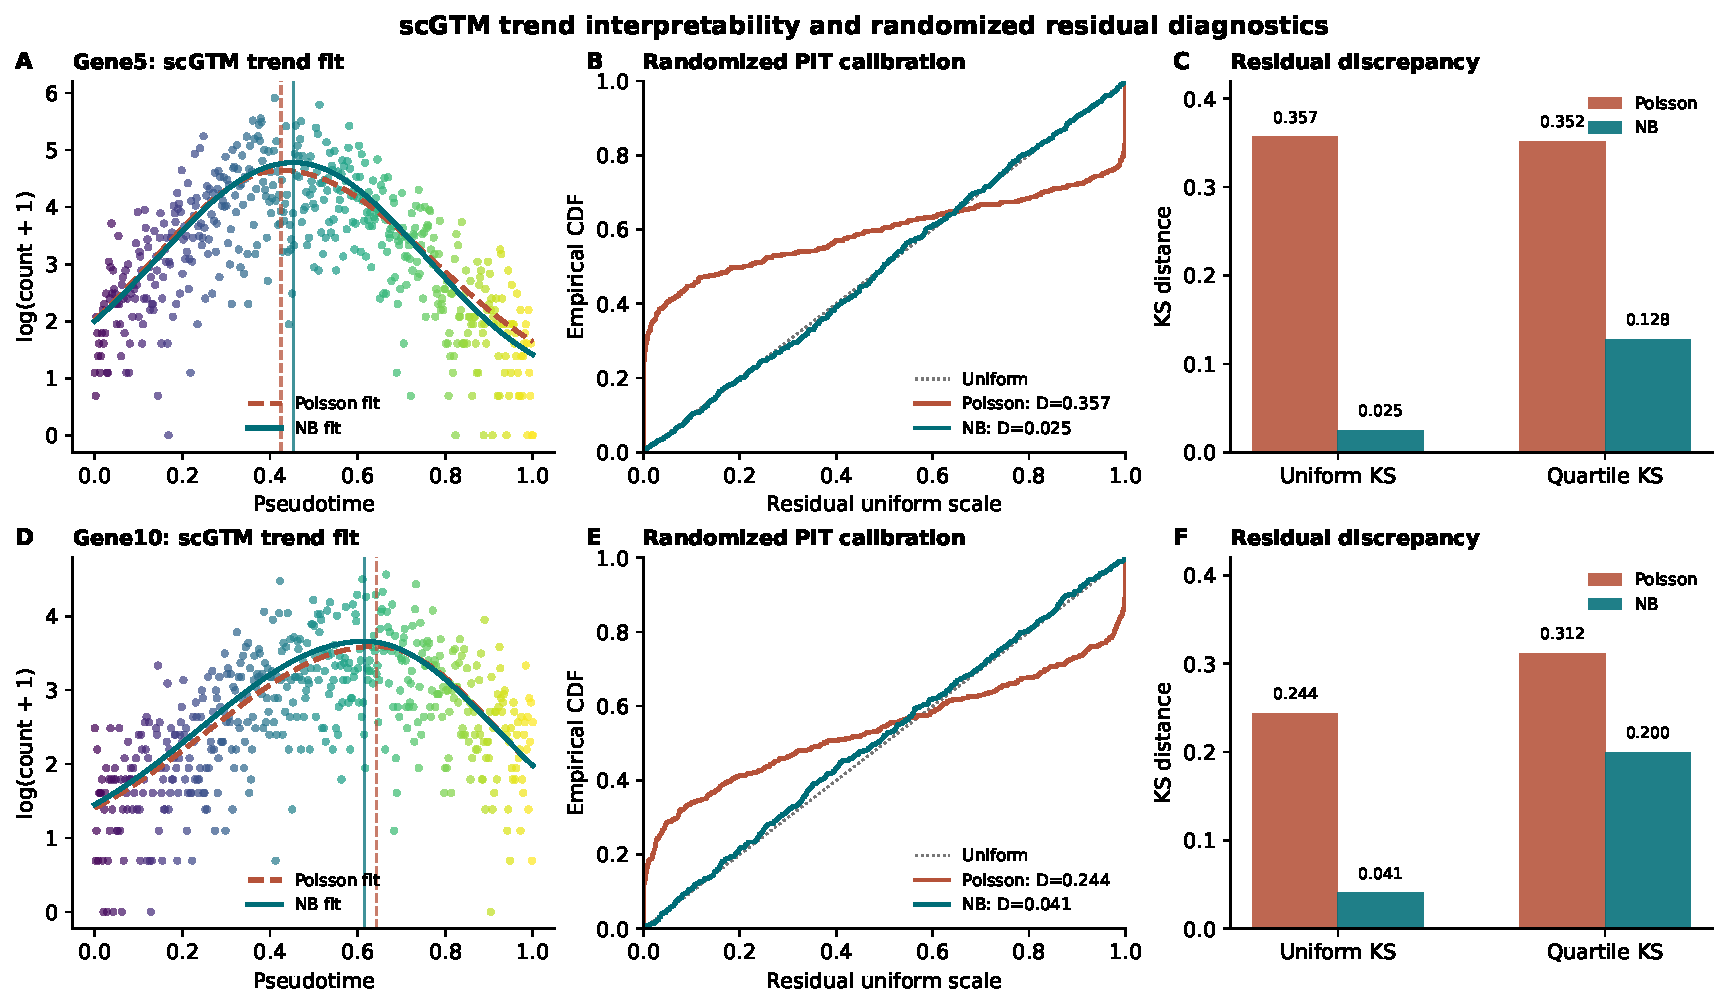
\includegraphics[width=\linewidth]{figs/scgtm_residual_calibration.pdf}
\caption{scGTM demonstration using two representative genes from a supplied
500-observation, 10-gene count matrix. Panels A and D show fitted Poisson and negative-binomial
(NB) scGTM trends on the pseudotime scale, with vertical lines marking the
estimated change time $t_0$. Panels B and E show randomized PIT residual ECDFs
against the uniform reference. Panels C and F compare the one-sample uniform
KS distance with the largest two-sample KS distance between pseudotime
quartiles. The uniform $p$-values reported in Table~\ref{tab:scgtm-example}
are descriptive because the trend margins were fitted.}
\label{fig:scgtm-residual-calibration}
\end{figure}

\begin{table}[!htbp]
\centering
\scriptsize
\caption{scGTM residual diagnostics for representative genes and the full
10-gene demonstration. The fitted change time $t_0$ and trend strengths $k_1,k_2$
describe the trajectory; $D$ is the uniform KS distance and Bin KS is the
largest two-sample distance between pseudotime quartiles. Simple $p$-values
are descriptive because the margins were fitted. All genes use the hill-shaped
trend without the package's valley transformation. Supplementary Appendix H
identifies the complete gene-level results.}
\label{tab:scgtm-example}
\setlength{\tabcolsep}{3pt}
\begin{tabular}{@{}llccccccc@{}}
\toprule
Gene & Margin & $t_0$ & $k_1$ & $k_2$ & $\phi$ & $D$ & Simple $p$ & Bin KS\\
\midrule
\texttt{Gene5} & Poisson & 0.425 & 4.995 & 3.554 & -- & 0.357 & $1.28\times10^{-57}$ & 0.352\\
 & NB & 0.454 & 4.593 & 4.802 & 1.980 & 0.025 & 0.905 & 0.128\\
\texttt{Gene10} & Poisson & 0.643 & 2.790 & 5.282 & -- & 0.244 & $1.03\times10^{-26}$ & 0.312\\
 & NB & 0.616 & 2.958 & 4.658 & 3.052 & 0.041 & 0.373 & 0.200\\
\addlinespace
\multicolumn{2}{@{}l}{10-gene aggregate} &
\multicolumn{7}{>{\raggedright\arraybackslash}p{0.66\linewidth}@{}}{median $D$: Poisson 0.278, NB 0.035; NB lower in 10/10 genes; median Bin KS decrease 0.112}\\
\bottomrule
\end{tabular}
\end{table}

\paragraph{scGTM trend-model demonstration}
We use the count matrix distributed in the scGTM software demonstration,
comprising 500 observations with supplied pseudotimes, and fit its first
10 genes. This software example is not treated as independent biological
validation; its generating mechanism is not documented in the source
repository. Supplementary Appendix H identifies the input and software version.
Figures~\ref{fig:scgtm-residual-calibration} and
\ref{fig:scgtm-workflow} and Table~\ref{tab:scgtm-example}
connect the residual calibration principle to an interpretable pseudotime trend
model. We retain the scGTM package's particle-swarm fitting algorithm for this
example. The fit reports a change time $t_0$ and side-specific trend
strengths $k_1$ and $k_2$, giving a compact summary of the fitted
gene-expression trajectory. The randomized residuals ask a different question:
after the trend has been fitted, do the conditional count margins still look
adequate on the uniform scale? In this demonstration, the Poisson trend captures an
interpretable trajectory but leaves strong residual non-uniformity, while the
negative-binomial trend greatly reduces both the one-sample residual
discrepancy and the pseudotime-bin discrepancy. Across the 10 fitted demo
genes, the NB margin has a smaller one-sample residual KS distance than the
Poisson margin for all 10 genes; the median residual KS distance decreases
from 0.278 to 0.035, the median quartile-indexed KS distance decreases by
0.112, and the median negative log-likelihood decreases by 1176.5. The
comparison illustrates why trend interpretability and distributional
adequacy should be assessed separately. These descriptive comparisons do not
establish nominal test calibration for the scGTM fitting procedure.

\begin{figure}[!htbp]
\centering
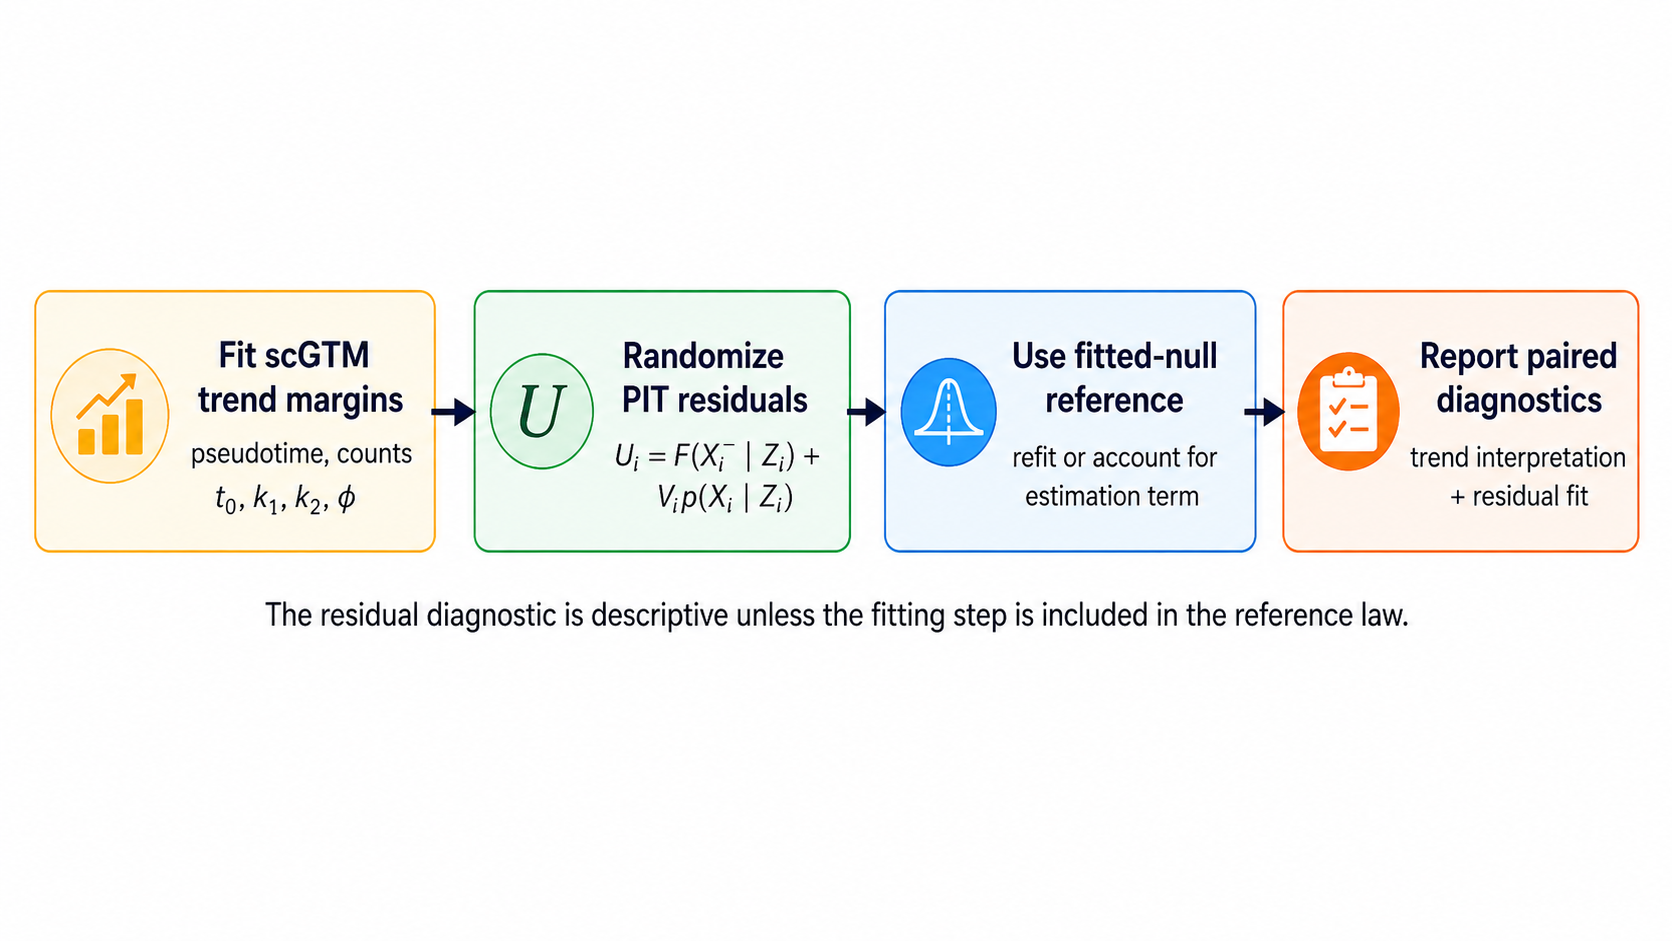
\includegraphics[width=\linewidth,trim=0 210 0 210,clip]{figs/scgtm_calibration_workflow.png}
\caption{Operational scGTM residual-diagnostic workflow. The trend parameters
summarize the fitted pseudotime trajectory, while randomized PIT residuals
diagnose the fitted conditional count margin. The residual statistic is
descriptive unless the reference law also includes the same fitting step, for
example through a refitted bootstrap.}
\label{fig:scgtm-workflow}
\end{figure}

\begin{figure}[t]
\centering
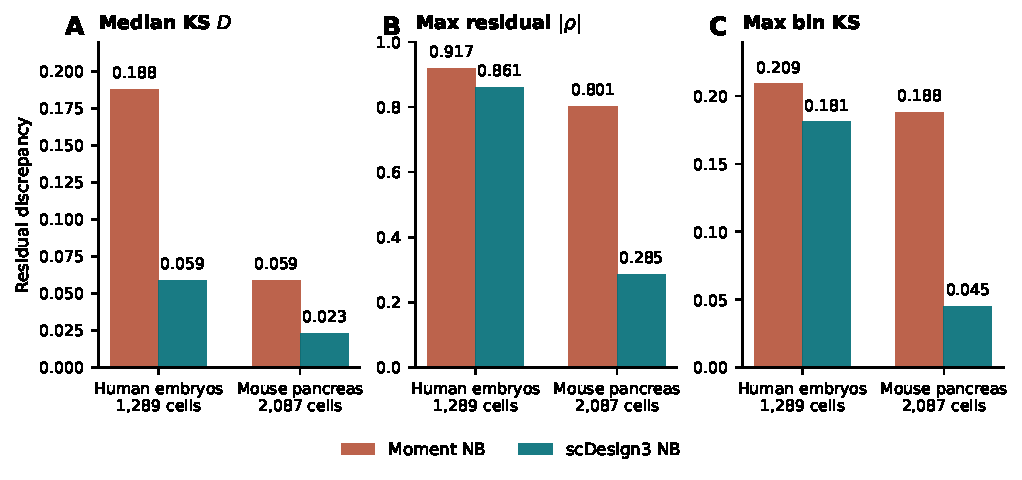
\includegraphics[width=\linewidth]{figs/scdesign3_residual_diagnostics.pdf}
\caption{Residual diagnostics for human preimplantation embryos (1,289 cells,
10 genes; E-MTAB-3929) and mouse pancreatic endocrinogenesis (2,087 cells,
100 genes; GSE132188), using the subsets distributed with scDesign3.
Moment negative-binomial margins are compared with scDesign3 conditional
negative-binomial fits. (A) Median gene-wise uniform KS distance.
(B) Maximum absolute pairwise residual correlation.
(C) Maximum two-sample KS distance between pooled residuals in pseudotime
quartiles. Panels B and C are descriptive summaries, not calibrated joint
tests.}
\label{fig:scdesign3-residual-diagnostics}
\end{figure}

\Needspace{5\baselineskip}
\subsection{Real-Data Applications}
\label{sec:real-data}

\paragraph{Mouse pancreatic endocrinogenesis}

The pancreatic data originate from a mouse pancreatic endocrinogenesis study
and are publicly available as
\href{https://www.ncbi.nlm.nih.gov/geo/query/acc.cgi?acc=GSE132188}{GEO GSE132188}.
The processed trajectory data are
distributed through scVelo and used by the scDesign3 tutorial
\citep{bastidasponce2019pancreas,bergen2020scvelo,song2024scdesign3}. The
tutorial retains 2,087 cells and the top 100 highly variable genes with matched
pseudotime. Figure~\ref{fig:scdesign3-residual-diagnostics} compares
simple moment margins with scDesign3 conditional negative-binomial margins.
The conditional fit reduces the median gene-wise KS distance from 0.059 to
0.023, the maximum absolute residual correlation from 0.801 to 0.285, and the
maximum pseudotime-quartile KS distance from 0.188 to 0.045.

We then apply Algorithm~\ref{alg:workflow} to the first 10 highly variable
genes in the package ordering. For each gene, we fit the scDesign3 conditional
negative-binomial margin, simulate 1,999 conditional count vectors at the
observed pseudotimes, and repeat the fit using scDesign3's per-gene regression
function, \texttt{fit\_marginal}. Fresh randomized PIT residuals are generated
and the gene-wise KS statistic is recomputed after each fit. All 19,990
bootstrap fits succeeded. Table~\ref{tab:pancreas-refit} compares the naive
and refitted tail probabilities for the same observed residuals. For
\textit{Chga}, the naive uniform $p$-value is 0.0237 and the refitted value is
0.0020. Both are below 0.05 before multiplicity correction, but only the
refitted value remains below 0.05 after Holm correction over the 10-gene
panel (0.0160, versus 0.1657 for the naive values). This difference concerns
the reference distribution of the residual statistic, not an improvement in
the observed fitted curve. Five genes, \textit{Pyy}, \textit{Iapp},
\textit{Rbp4}, \textit{Chga}, and \textit{Nnat}, have Holm-adjusted refitted
$p<0.05$.

This analysis conditions on the supplied pseudotimes and gene ordering.
Neither trajectory estimation nor highly variable gene selection is repeated
in the bootstrap. It therefore assesses the selected conditional margins,
without accounting for uncertainty in those upstream steps. The refitted
bootstrap reference distributions are empirical approximations: the
simulator-specific conditions for the asymptotic result have not been
established here. Table~\ref{tab:scdesign-simulations} supplies a focused
finite-sample check of the same spline-margin configuration under a specified
fixed-design null, not a validation of the full pancreatic preprocessing
workflow. Supplementary Appendix H reports conditional Monte Carlo
intervals and the fixed randomization protocol. A single observed
randomization is used per gene; sensitivity to that randomization is not
assessed by increasing the number of bootstrap draws.

\begin{table}[!htbp]
\centering
\scriptsize
\caption{Refitted marginal calibration for the first 10 highly variable genes
in the 2,087-cell pancreatic endocrinogenesis data. Each refitted value uses
$B=1,999$ complete scDesign3 conditional-margin refits. Holm correction is
over all 10 genes. The minimum attainable Monte Carlo $p$-value is 0.0005.}
\label{tab:pancreas-refit}
\setlength{\tabcolsep}{5pt}
\begin{tabular}{@{}lccccc@{}}
\toprule
Gene & KS $D$ & Naive $p$ & Refit $p$ & Holm $p$ & Refit 95\% cutoff\\
\midrule
\textit{Pyy}  & 0.0300 & 0.0472 & 0.0025 & 0.0160 & 0.0225\\
\textit{Iapp} & 0.0332 & 0.0203 & 0.0020 & 0.0160 & 0.0239\\
\textit{Chgb} & 0.0206 & 0.3395 & 0.1225 & 0.3675 & 0.0235\\
\textit{Rbp4} & 0.0439 & 0.0006 & 0.0005 & 0.0050 & 0.0232\\
\textit{Spp1} & 0.0241 & 0.1763 & 0.0715 & 0.3075 & 0.0250\\
\textit{Chga} & 0.0326 & 0.0237 & 0.0020 & 0.0160 & 0.0229\\
\textit{Cck}  & 0.0167 & 0.6068 & 0.2885 & 0.3675 & 0.0217\\
\textit{Ins1} & 0.0224 & 0.2479 & 0.1520 & 0.3675 & 0.0263\\
\textit{Nnat} & 0.0432 & 0.0008 & 0.0005 & 0.0050 & 0.0233\\
\textit{Ins2} & 0.0263 & 0.1105 & 0.0615 & 0.3075 & 0.0272\\
\bottomrule
\end{tabular}
\end{table}

\paragraph{Human preimplantation embryos}
The human preimplantation embryo data were reported by
\citet{petropoulos2016embryos} and are available under
\href{https://www.ebi.ac.uk/biostudies/arrayexpress/studies/E-MTAB-3929}{E-MTAB-3929}.
We use the scDesign3 subset containing 1,289 cells and 10 genes.
All supplied cell identifiers and developmental-stage labels match the
public sample annotation. The five groups represent embryonic days 3--7,
not five inferred cell types; the supplied pseudotime ranges from 0 to 1.
The conditional margin reduces
the median gene-wise KS distance from 0.188 to 0.059, but the maximum absolute
pairwise residual correlation remains 0.861. This contrast illustrates
Proposition~\ref{prop:copula-blind-spot} and
Remark~\ref{rem:conditional-residuals}: marginal uniformity, residual
dependence summaries, and covariate-indexed residual structure are different
diagnostic targets. Supplementary Appendix H specifies the package objects,
provenance check, and numerical files in Online Resource 1.

\paragraph{Translational case study: IMvigor210 baseline PBMCs}
We next analyze public integer UMI-count matrices from the baseline PBMC
single-cell experiment reported by \citet{yuen2020il8}. The 10 patients, five
responders and five nonresponders, were treated in the IMvigor210 atezolizumab
program; the relevant cohort is registered as NCT02108652 and the single-cell
matrices are deposited as GEO GSE145281. We independently retain cells with at
least 500 UMIs, 200--6000 detected genes, and mitochondrial fraction at most
0.20. This leaves 24,134 of 26,749 candidate count-matrix columns. Response
labels are used only to describe the samples, not to test treatment efficacy or
construct a response classifier.

For a source-motivated panel fixed before residual fitting from the source
study's IL-8 and antigen-presentation analysis, we fit the transparent working margin
\[
Y_{ijg}\sim\operatorname{NB}(\mu_{ijg},r_g),\qquad
\mu_{ijg}=L_{ij}\lambda_{jg},
\]
where $L_{ij}$ is the observed library-size offset for cell $i$ in patient $j$,
$\lambda_{jg}$ is a patient-specific rate, and $r_g$ is a shared gene-specific
dispersion. We estimate each rate by its exposure-adjusted patient mean and
$r_g$ by the pooled NB2 moment equation; the same rule is repeated in every
bootstrap sample. The diagnostic statistic
\[
S_g=\max_{1\le j\le10}\sqrt{n_j}\,D_{jg}
\]
uses the largest patient-stratified randomized-PIT KS discrepancy on its
null fluctuation scale, avoiding dilution of a patient-specific discrepancy
in a pooled empirical distribution. Each of $B=9,999$ bootstrap replicates holds
the patient and library-size design fixed, simulates counts, re-estimates
$\lambda_{jg}$ and $r_g$, generates fresh randomizers, and recomputes $S_g$. A
fixed-parameter comparator omits only the re-estimation step.

To investigate the discrepancies under this shared-dispersion model, we also
fit an exploratory extension with patient-specific dispersions $r_{jg}$.
The mean model, count data, QC rules, and complete 10-gene panel are unchanged.
This extension allows patient-to-patient differences in conditional variance
without introducing unverified cell-type annotations. Its moment estimators
are refitted in each of a separate set of 9,999 bootstrap samples per gene.
The extension and its simulation size were fixed before computation.

The working reference assumes independent cells conditional on patient and
the retained library-size offsets. Patient stratification does not account
for arbitrary within-patient dependence. Because library sizes and QC are
derived from the expression data and then held fixed, this is a conditional
working-model check, not a calibration result for the full preprocessing or
patient-sampling procedure. A rejection can reflect a failure of these sampling
assumptions as well as an inadequate count margin.

\begin{figure}[t]
\centering
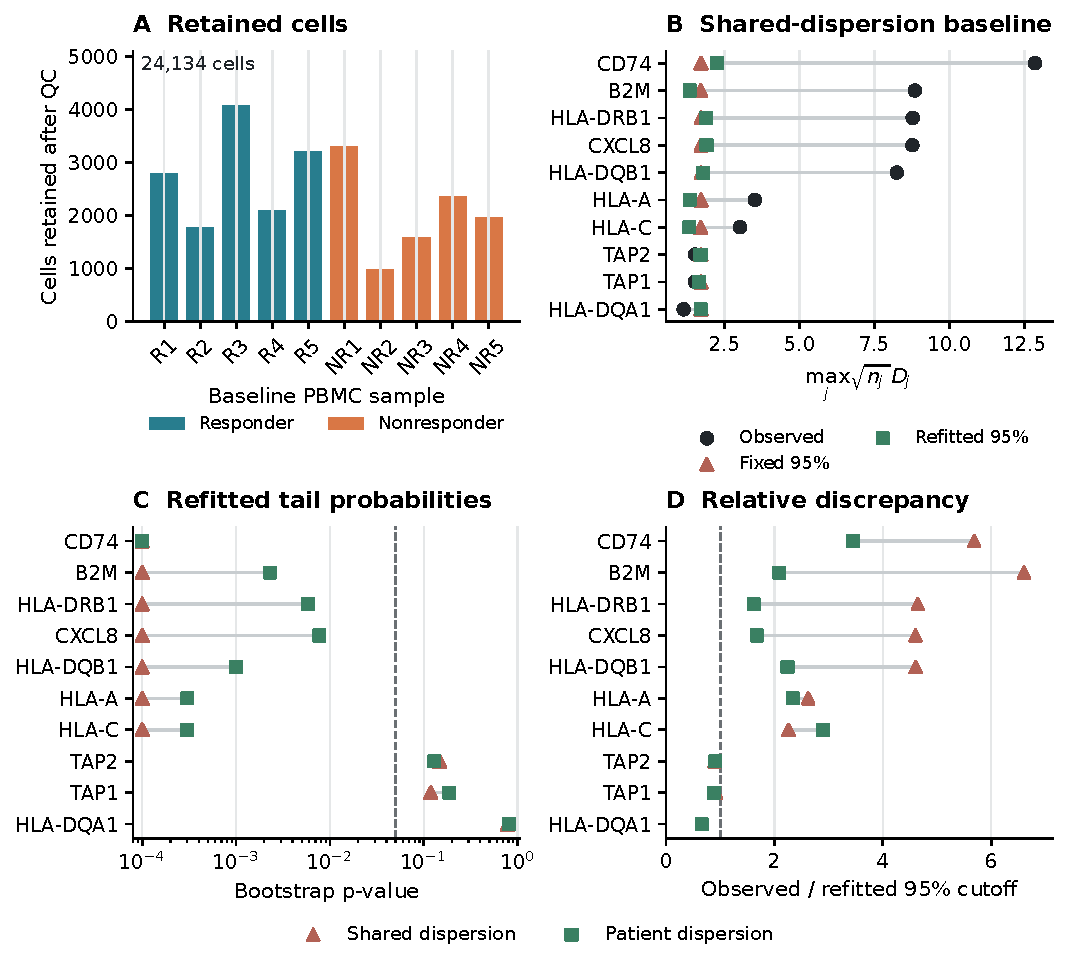
\includegraphics[width=\linewidth]{figs/imvigor210_residual_diagnostics.pdf}
\caption{Public IMvigor210 baseline-PBMC residual diagnostics (GEO GSE145281;
NCT02108652). Panel A shows cells retained after independent QC; response labels
are descriptive only. Panel B compares the observed patient-stratified statistic
$S_g$ with 95\% fixed-parameter and refitted-bootstrap cutoffs for the
shared-dispersion model. Panel C compares plus-one refitted-bootstrap
$p$-values under shared and patient-specific dispersions. Panel D compares
the observed statistic divided by each model's refitted 95\% cutoff. Dashed
lines in C and D mark unadjusted 5\% thresholds, not multiplicity-adjusted
decisions. Each model uses $B=9,999$ replicates per gene. The gene panel was
fixed before residual fitting from the source study's CXCL8 and
antigen-presentation focus. Supplementary Appendix G gives both models'
numerical results, Holm adjustments, and Monte Carlo intervals.}
\label{fig:imvigor210-diagnostics}
\end{figure}

Figure~\ref{fig:imvigor210-diagnostics} shows strong inadequacy of this simple
working margin for \textit{CXCL8}, \textit{B2M}, \textit{CD74},
\textit{HLA-A}, \textit{HLA-C}, \textit{HLA-DQB1}, and
\textit{HLA-DRB1}: all seven refitted $p$-values equal the attainable minimum
0.0001 and equal 0.0010 after Holm correction over the 10-gene panel. Each has
zero exceedances in 9,999 draws; the upper endpoint of its conditional 95\%
Monte Carlo interval for the unadjusted tail probability is 0.000369.
The refitted values for
\textit{HLA-DQA1}, \textit{TAP1}, and \textit{TAP2} are 0.7785, 0.1188,
and 0.1470, respectively.

Allowing patient-specific dispersion produces a mixed improvement. For
\textit{CXCL8}, $S_g$ decreases from 8.768 to 5.403 and the refitted $p$-value
increases to 0.0077; for \textit{B2M}, the corresponding changes are 8.849 to
3.275 and $p=0.0023$. Their mean fitted log scores also increase. However,
the observed discrepancies increase for \textit{CD74} and \textit{HLA-C},
and the fitted log score decreases for \textit{HLA-DQB1}. All seven originally
flagged genes retain Holm-adjusted $p<0.05$ under the extension (range
0.0010--0.0308). Neither candidate rejects the other three genes after
adjustment. All 199,980 bootstrap refits across both models succeed.
Patient-specific dispersion alone does not remove these discrepancies;
Appendix G reports the complete comparison.

\begin{table}[t]
\centering
\scriptsize
\caption{Summary of diagnostic targets, numerical evidence, and supported
interpretations.}
\label{tab:evidence-summary}
\begin{tabular}{@{}>{\raggedright\arraybackslash}p{0.24\linewidth}>{\raggedright\arraybackslash}p{0.39\linewidth}>{\raggedright\arraybackslash}p{0.29\linewidth}@{}}
\toprule
Target & Key evidence & Supported interpretation and limitation\\
\midrule
Fitted margins need fitted-null calibration &
NB simulation: naive rejection 0.000; refitted rejection 0.040--0.062 across
$n=250$--10,000 &
The fitted workflow, not the simple-null bridge, is the relevant reference;
synthetic count margin.\\
\addlinespace
Marginal KS misses copula errors &
Wrong copula $\rho=0.50$: marginal KS 0.054/0.050; residual-correlation diagnostic 0.663 &
Single-gene marginal residuals do not validate dependence; two-gene copula
illustration.\\
\addlinespace
scGTM trend fit and residual fit are distinct &
10 demo genes: median residual KS 0.278 to 0.035; NB lower in 10/10 genes &
Trend parameters and residual adequacy should be reported together; package
demo matrix.\\
\addlinespace
Pancreatic conditional margins require fitted calibration &
\textit{Chga}: naive $p=0.0237$, refitted $p=0.0020$; 19,990/19,990 bootstrap fits succeeded &
The reference changes the tail probability and multiplicity-adjusted decision;
not validation of the fitted copula.\\
\addlinespace
Clinical PBMC margins remain falsifiable after calibration &
IMvigor210: 7/10 genes have Holm $p=0.0010$ under shared dispersion and
$p\le0.0308$ with patient-specific dispersion &
Allowing patient-specific dispersion does not remove the seven discrepancies;
the model comparison is exploratory, not a treatment-response analysis.\\
\addlinespace
Marginal improvement is not joint calibration &
Human embryos: median KS 0.188 to 0.059, but residual correlation remains 0.861 &
Diagnostics must separate marginal, dependence, and covariate-indexed targets;
10-gene developmental subset.\\
\bottomrule
\end{tabular}
\end{table}

\section{Applicability and Computational Considerations}
\label{sec:applicability}

The asymptotic result in Section~\ref{sec:theory} is most directly applicable
to regular finite-dimensional fits. Modern single-cell tools differ
substantially in whether their estimators and residual maps satisfy those
conditions. Table~\ref{tab:tool-regularity} therefore separates settings in
which the assumptions can plausibly be verified from settings in which a
refitted simulation is only an empirical, workflow-specific approximation.
These conditions determine the inferential interpretation of the diagnostic.

\begin{table}[!htbp]
\centering
\scriptsize
\caption{Relationship between representative single-cell workflows and the
regularity conditions used by the randomized residual process. ``Potentially
verifiable'' means that model- and algorithm-specific verification is still
required.}
\label{tab:tool-regularity}
\setlength{\tabcolsep}{3pt}
\begin{tabular}{@{}>{\raggedright\arraybackslash}p{0.16\linewidth}>{\raggedright\arraybackslash}p{0.27\linewidth}>{\raggedright\arraybackslash}p{0.24\linewidth}>{\raggedright\arraybackslash}p{0.25\linewidth}@{}}
\toprule
Workflow & Relevant fitted object & Status of stated theory & Recommended interpretation\\
\midrule
scGTM & Low-dimensional gene-wise trajectory and count-margin parameters & Potentially verifiable for fixed pseudotime, interior parameters, and a stable optimum; estimated pseudotime requires an additional expansion & Verify analytic or bootstrap conditions; otherwise assess the refitted reference empirically.\\
\addlinespace
scDesign2 & Gene-wise margins and an estimated Gaussian copula & Margin theory may be checked gene by gene; increasing-dimensional copula estimation is not covered by the fixed-dimensional statement & Calibrate marginal and dependence statistics separately and refit both components relevant to each statistic.\\
\addlinespace
scDesign3 & Smooth conditional margins, distribution selection, and dependence estimation & Smoothing, model selection, and increasing parameter dimension make asymptotic linearity and the plug-in remainder nonautomatic & Treat the full refitted workflow as empirical calibration unless sufficient conditions are established for the selected fit.\\
\addlinespace
scVI-type models & Variational neural estimation with latent variables and many parameters & Not covered directly by the stated finite-dimensional regularity conditions & Use held-out predictive checks or a model-specific simulation study; describe a refitted bootstrap as heuristic unless separately justified.\\
\addlinespace
Foundation models (e.g., scGPT) & Learned representations or predictions without an explicit fitted count CDF & A randomized PIT residual may not be defined & Outside the direct scope of this method until a probabilistic count reference and diagnostic target are specified.\\
\bottomrule
\end{tabular}
\end{table}

Let $C_{\rm fit}(n,G)$ denote the cost of fitting the model to $n$ cells and
$G$ genes, and let $C_S(n,G)$ be the cost of constructing residuals and the
chosen statistic. A serial refitted bootstrap with $B$ samples costs
\[
O\{(B+1)[C_{\rm fit}(n,G)+C_S(n,G)]+B C_{\rm sim}(n,G)\},
\]
where $C_{\rm sim}$ denotes the cost of generating one bootstrap data set.
Bootstrap replicates are conditionally independent, so they can run on
separate workers. Residuals and gene-wise statistics can also be streamed so
that all $n\times G$ residuals need not be stored simultaneously.
Table~\ref{tab:scalability} reports measured times for the observed procedure
and one bootstrap replicate.

The conditional-regression study comprises $4\times500=2,000$ outer
samples and $4\times500\times199=398,000$ bootstrap margin refits,
or 400,000 fits including the observed samples. The timed four-scenario
run took 3,122.6 seconds (52.0 minutes) on an Apple M1 Max CPU
(10 cores), with 64\,GiB memory and macOS 26.5.2, using four worker
processes and one fitting core per worker. The largest conditional sample
has 2,087 cells: the refit total describes computational workload, not
validation at a 398,000-cell sample size. Supplementary Appendix H.6
reports the software environment and task-level timings for these
simulations, the 19,990 pancreatic refits, and the 199,980 clinical
PBMC refits. Summed task times are distinguished from elapsed wall time.

\begin{table}[!htbp]
\centering
\scriptsize
\caption{Single-worker CPU scalability check for a lightweight 10-gene
moment-NB workflow on the machine described in the text. Times are medians
of five sequential repetitions, after an excluded warm-up.
``Observed'' includes generation of the synthetic counts, fitting,
randomized residual construction, and the KS statistic; ``one refit'' repeats
those operations on one bootstrap data set. The projected time for $B=199$
is calculated from the two median timings and assumes serial execution;
199 complete refits were not timed. The memory column is an analytic
baseline of $24n$ bytes for three
64-bit arrays, not measured peak memory; it excludes additional temporary
arrays, interpreter overhead, and input-matrix storage. These timings do not
represent the substantially more expensive scDesign3 fit.}
\label{tab:scalability}
\setlength{\tabcolsep}{4pt}
\begin{tabular}{@{}rccccc@{}}
\toprule
Cells & Genes & Observed (s) & One refit (s) & Projected $B=199$ (min) & Array baseline (MiB)\\
\midrule
\inputresultrows{results/computational_reporting/lightweight_table_rows.tex}
\bottomrule
\end{tabular}
\end{table}

Table~\ref{tab:scalability} shows approximately linear observed runtime over
the tested range, up to one million cells. Moment fitting is linear in $n$,
whereas the implementation sorts residuals for KS evaluation, with
$O(n\log n)$ comparison-sorting cost per gene. This is a feasibility check, not
evidence that a full scDesign3 or variational model can be refitted at the same
rate. For expensive models, wall time is dominated by $C_{\rm fit}$; parallel
bootstrap workers can reduce elapsed time without reducing the number of
fits; no parallel speedup ratio is estimated here. Appendix H.6 specifies
the timing boundaries and retains all five repetitions.

For models fitted by stochastic optimization, such as the scGTM likelihood
applications in \citet{cui2024natureinspired}, the initialization rule,
parameter bounds, stopping criterion, and search budget are part of the
fitting procedure. A refitted reference should use the same rules as the
observed fit, including the treatment of optimizer randomization. Repeating
these rules does not itself establish bootstrap consistency: the estimator
must still satisfy the stability and asymptotic conditions stated above.

\Needspace{4\baselineskip}
For smooth, low-dimensional models, the covariance expansion suggests a
faster alternative to complete refitting. For randomized residuals, define
\[
q(u)=\mathbf 1\{T_{F_{\theta_0}}(X,V)\le u\}-u,
\qquad a(u)=\dot G_{\theta_0}(u).
\]
The fitted residual limit has covariance
\[
K(u,v)=\mathbb E\bigl[\{q(u)+a(u)^T\psi_{\theta_0}(X)\}
\{q(v)+a(v)^T\psi_{\theta_0}(X)\}\bigr].
\]
Estimating $K$ on a threshold grid and simulating centered Gaussian vectors
gives an approximate reference for the maximum absolute residual process.
This retains the covariance between the empirical and estimation terms;
simply adding independent parameter noise would not. It avoids repeated
fitting, but requires consistent derivatives, influence functions, and
covariance estimates, together with control of grid approximation error.
We describe this alternative analytically; no Gaussian-reference benchmark
is reported in this study. Sample splitting or cross-fitting can reduce reuse of the same cells,
but changes the inferential target and does not by itself remove uncertainty in
the fitted reference distribution.

\section{Discussion}
The central distinction is operational. If a discrete margin is known and the
randomized distributional transform is used, the ordinary uniform KS reference
is valid. If the margin is estimated from the cells being checked, the fitting
step changes the residual process and must be represented in the reference
law.

This distinction matters for fitted-model validation. A naive KS cutoff can be
severely conservative under fitted models, as shown in Table~\ref{tab:nb-scale}.
Under the regularity conditions described above, the remedy is to calibrate
the statistic against the fitted workflow:
simulate from the fitted model, refit the model in each simulated dataset, and
recompute the same residual statistic. When the bootstrap analogues of the
expansion hold, the refitted bootstrap targets the plug-in empirical-process
limit rather than the simple-null bridge.

The pancreatic analysis shows why the distinction matters beyond null
simulations. Refitting changes some gene-level $p$-values enough to alter the
multiplicity-adjusted diagnostic decision. The simulation demonstrates severe
conservatism for the tested moment-NB fit; it does not establish the direction
of error for every fitted model. In the pancreatic example, some values also
reach the Monte Carlo floor, which limits comparisons between very small
tail probabilities.

The IMvigor210 analysis adds a clinically sourced stress test. Even after the
reference procedure repeats the fitted patient-and-depth conditional margin,
seven prespecified genes show discrepancies far beyond the refitted reference.
The patient-specific-dispersion extension improves some fitted summaries but
leaves all seven genes flagged after within-model Holm correction. Thus,
relaxing shared dispersion alone is insufficient. The present analysis does
not identify whether remaining discrepancies arise from cell-state mixtures,
within-patient dependence, or other aspects of the count model. Its model
comparison is exploratory and its log scores are in-sample summaries.
This is evidence against the conditional working references, not evidence about
atezolizumab efficacy or the published IL-8 biomarker claim. The distinction is
important in translational analyses: reference calibration controls how a
diagnostic is judged, whereas biological interpretation requires a model and
sampling design appropriate to the clinical question.

The contribution is broader than a package-specific diagnostic but narrower
than a universal validation framework. For any workflow with an explicit
fitted discrete or conditional distribution, the analyst can specify the
residual map, identify whether its reference was fixed or fitted, and construct
a reference for the same statistic under the same fitting algorithm. For latent-variable,
foundation, or black-box generators, a probabilistic count reference and a
refitting scheme must first be defined before KS-style residual calibration can
be claimed.

The copula result adds a second warning. A gene-wise KS diagnostic is useful for
checking marginal count calibration, but it cannot validate the dependence
structure of a scDesign2-type simulator. Correlation and copula fit require
joint residual diagnostics. For conditional single-cell trend-model and simulator diagnostics,
the same logic suggests residual processes indexed jointly by residual
thresholds and cell covariates such as pseudotime, modality, batch, or spatial
region.

The supplementary appendix gives the fixed-null crossing formulas, an optional
geometric interpretation, and the deferred proofs. For applications, the
essential steps are those in Algorithm~\ref{alg:workflow}: specify the target,
construct the residual statistic, and include the relevant estimation steps
in its reference procedure. Report the statistic, calibration method,
Monte Carlo resolution, and assumptions together. In pseudotime analyses,
trend parameters describe the fitted trajectory, while residual diagnostics
assess departures from the conditional count model. These outputs answer
different questions and should be interpreted together.

\section*{Statements and Declarations}

\paragraph{Declaration of generative AI and AI-assisted technologies in the writing process}
During the preparation of this work the authors used OpenAI's ChatGPT/Codex
to assist with language editing, analysis-code drafting, LaTeX formatting,
and consistency checks.
After using this tool, the authors reviewed and edited the content as needed
and take full responsibility for the content of the publication.

\paragraph{Competing interests}
Yihao Li is affiliated with Genentech and Zhuang Liu is affiliated with Google.
The IMvigor210 analysis uses only public GEO data generated by the investigators
of the cited study; no proprietary Genentech data or sponsor support was used.
The authors declare no other competing interests directly related to this
article.

\paragraph{Funding}
No specific funding was reported for this work.

\paragraph{Author contributions}
Elvis Han Cui led the study conception, methodology, implementation,
manuscript drafting, and reproducibility packaging. Yihao Li and Zhuang Liu
contributed to methodological framing, interpretation, and manuscript review
and editing. All authors reviewed and approved the manuscript.

\paragraph{Ethics approval and consent to participate}
Not applicable. This methodological article uses synthetic data and publicly
available, previously published single-cell data.

\paragraph{Consent for publication}
Not applicable.

\paragraph{Data and code availability}
Online Resource 1 contains the editable manuscript sources, analysis scripts,
numerical tables, saved bootstrap statistics, figures, and software versions.
The README and Supplementary Appendix H give reproduction commands and
implementation details. A public reproducibility snapshot, including the
clean manuscript and supplement, is available at
\url{https://github.com/ElvisCuiHan/randomized-ks-calibration}.
The analyses reported here correspond to
\href{https://github.com/ElvisCuiHan/randomized-ks-calibration/releases/tag/v1.0.0}{release v1.0.0},
which includes a downloadable archive and per-file SHA-256 checksums.

The package examples use R's \texttt{InsectSprays} data and the scDesign3
objects \texttt{example\_count}, \texttt{example\_sce}, and
\texttt{pseudotime}. These provide the mouse pancreatic subset (GSE132188;
2,087 cells, 100 genes) and human embryo subset (E-MTAB-3929; 1,289 cells,
10 genes). Embryo cell identifiers and developmental stages were verified
against the public annotation, without reconstructing preprocessing or
pseudotime estimation. The scGTM demonstration uses its distributed count
matrix and trend-fitting function; Appendix H records the input path and
source commit.

The clinical case study uses the 10 public baseline-PBMC integer count
matrices in GEO GSE145281 from IMvigor210 (NCT02108652), retaining 24,134
cells after QC. Online Resource 1 includes source hashes, QC summaries,
complete results for both dispersion models, and a script to download the
source matrices. Clinical response labels are descriptive only. All 19,990
pancreatic and 199,980 PBMC refitted-bootstrap statistics are preserved,
together with seeds and conditional Monte Carlo summaries.



%\section{Acknowledgments}


\bibliographystyle{elsarticle-harv}

\bibliography{references, historical}

\end{document}
